\section{Implementation Details}


\begin{figure}[b]
    \centering
    {
        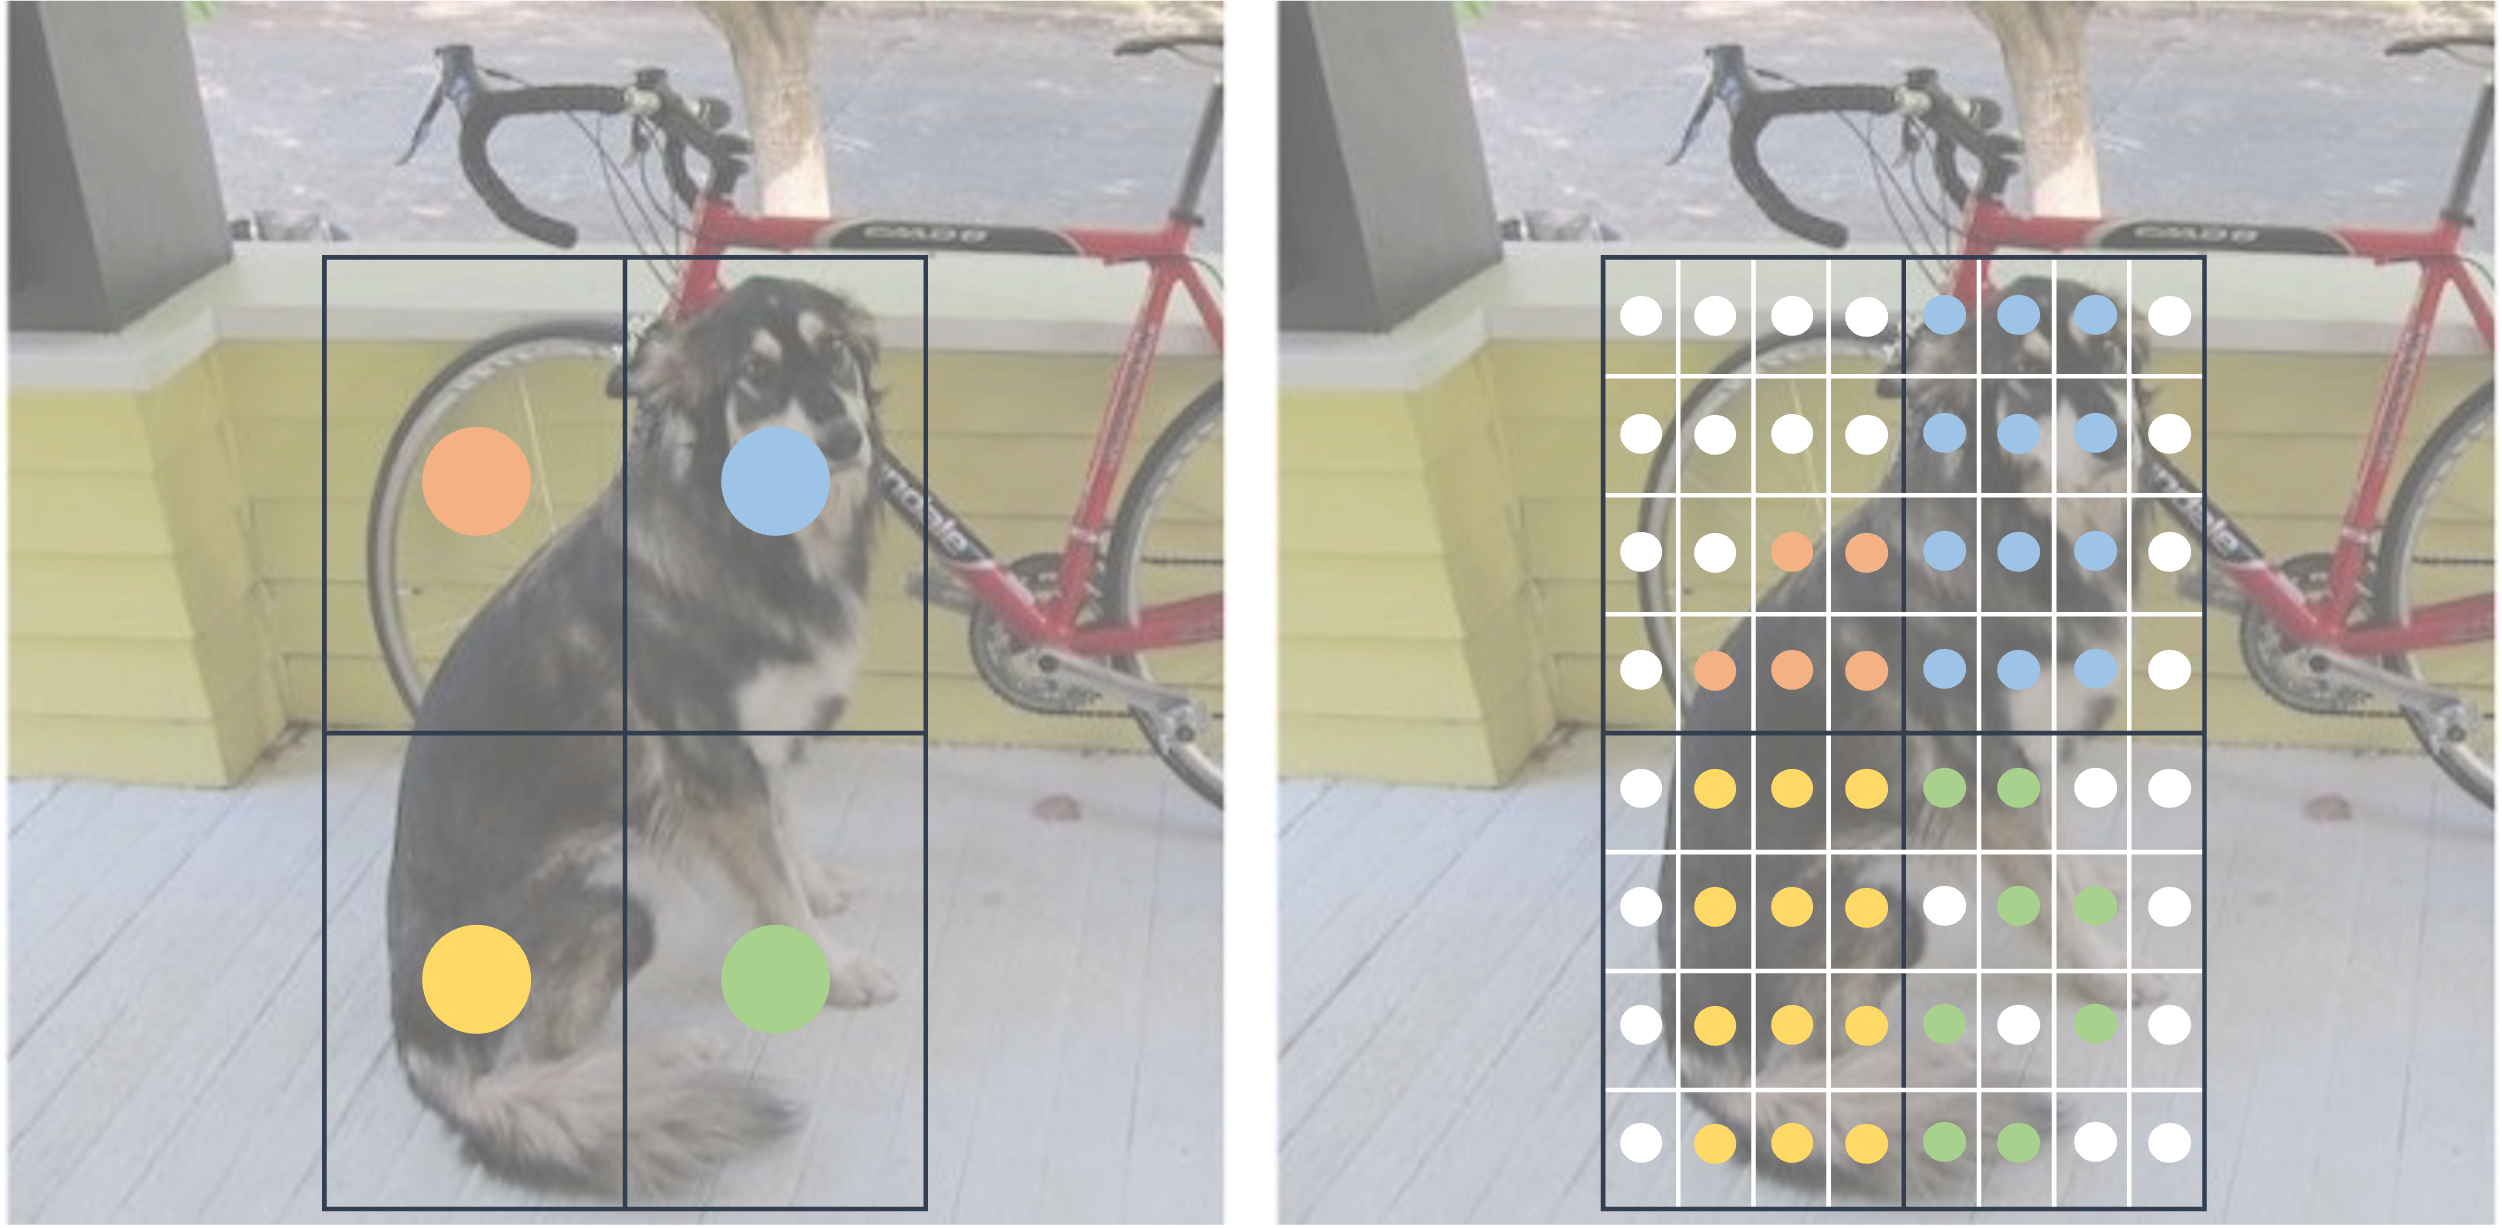
\includegraphics[width=\linewidth]{fig/attn_comp.png}
    }
    {
        \caption{\textbf{Masked Instance-Attention. Left:} The box-attention~\citep{nguyen2022boxer} which samples $2\times2$ grid features in the region of interest. \textbf{Right:} Our masked instance-attention for dense grid sampling that employs masking strategy to capture object boundary. The $2\times2$ attention scores are denoted in four colours and the masked attention score is shown in white.}
        \label{fig:masked_instance_attn}
    }%
\end{figure}

\boldparagraph{Masked Instance-Attention.} The masked instance-attention follows the grid sampling strategy of the box-attention in \cite{nguyen2022boxer}, but differs in the computation of attention scores to better capture objects of different shapes. To be specific, the region of interest $r'_i$ is divided into 4 bins of $2 \times 2$ grid, each of which contains a $\frac{m}{2} \times \frac{m}{2}$ grid features sampled using bilinear interpolation. Instead of assigning an attention weight to each feature vector, a linear projection ($\mathbb{R}^d \rightarrow \mathbb{R}^{2 \times 2}$) is adopted to generate the $2 \times 2$ attention scores for 4 bins. The $\frac{m}{2} \times \frac{m}{2}$ feature vectors within the same bin share the same attention weight. This is equivalent to the \textit{average} aggregation of feature values covered by each bin, which shows to reduce misalignments in RoIAlign~\citep{he2017maskrcnn}:
\begin{equation}
    \mathrm{head}_i = \sum_{k=0}^{2 \times 2} \sum_{j=0}^{\frac{m}{2} \times \frac{m}{2}} \frac{\alpha_k}{\frac{m}{2} \cdot \frac{m}{2}} \, v_{i_{k,j}},
\end{equation}
where $a_k$ is the attention weight corresponding to $k$-th bin and $v_{i_{k,j}}$ is the $j$-th feature vector inside $k$-th bin.

Inspired by \cite{cheng2022mask2former}, we utilize the mask prediction of the previous decoder layer $\mathcal{M}_q \in \mathbb{R}^{H_m \times W_m}$ corresponding to the object query $q$. Given the coordinates of grid features within the region of interest $r'_i$, we sample the corresponding mask scores using bilinear interpolation. The sampled mask scores are binarized with the 0.5 threshold before $\softmax$ in the attention computation. Note that in masked instance-attention, we sample the feature grid of $14\times14$.

\cref{fig:masked_instance_attn} shows the difference between box-attention~\citep{nguyen2022boxer} and masked instance-attention. By utilizing the mask prediction from previous decoder layer, masked instance-attention can effectively capture object of different shapes.


\boldparagraph{The creation of input features.} In \cref{fig:fpn_vs_ss}, we compare the creation of input features to detection head between SimpleFPN and our method. In \cite{li2022vitdet}, the multi-scale feature maps are created by different sets of convolution layers. Instead, \ours simply applies a deconvolution layer following by a GroupNorm layer~\citep{wu2018groupnorm}.


\begin{figure*}[t]
    \centering
    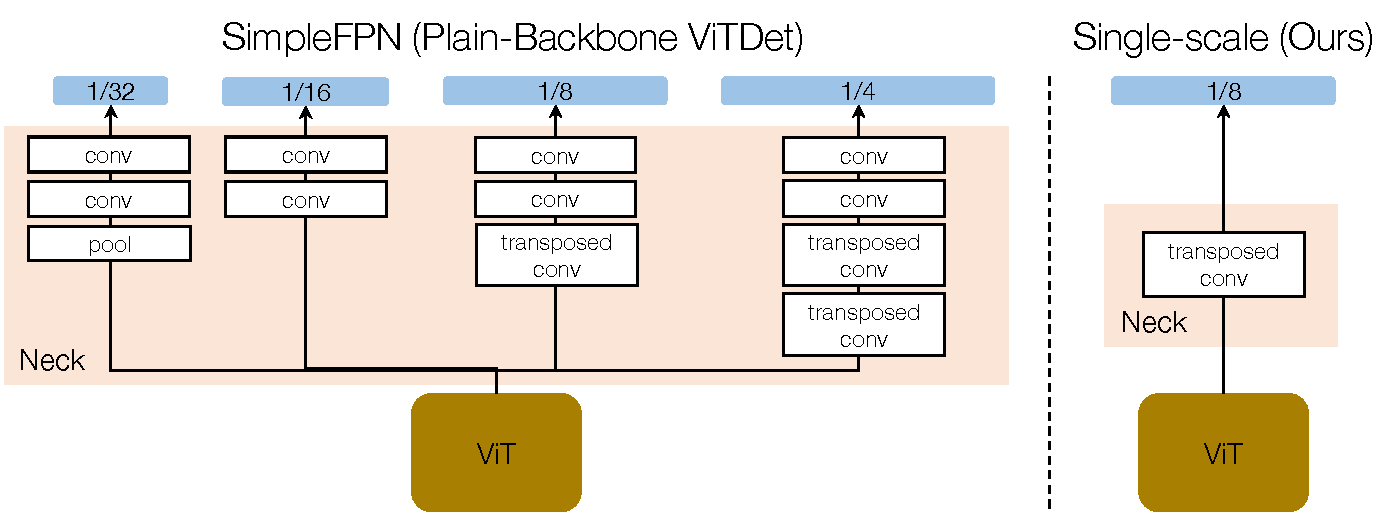
\includegraphics[width=0.8\linewidth]{fig/fpn_vs_ss_w_neck.pdf}\\
    \caption{
        \textbf{The creation of input features. Left:} The creation of feature pyramids from the last feature of the plain backbone, ViT, in SimpleFPN~\citep{li2022vitdet} where different stacks of convolutional layers are used to create features at different scales. \textbf{Right:} The design of our single-scale feature map with only one layer.
    }
    \label{fig:fpn_vs_ss}
\end{figure*}

\boldparagraph{Losses in training of \ours.} We use focal loss~\citep{lin2017focalloss} and dice loss~\citep{milletari2016vnet} for the mask loss: $\mathcal{L}_\text{mask} = \lambda_\text{focal}\mathcal{L}_\text{focal} + \lambda_\text{dice}\mathcal{L}_\text{dice}$ with $\lambda_\text{focal}=\lambda_\text{dice}=5.0$. The box loss is the combination of $\ell_1$ loss and GIoU loss~\citep{rezatofighi2019giou}, $\mathcal{L}_\text{box} = \lambda_{\ell_1}\mathcal{L}_{\ell_1} + \lambda_\text{giou}\mathcal{L}_\text{giou}$, with $\lambda_{\ell_1} = 5.0$ and $\lambda_\text{giou} = 2.0$. The focal loss is also used for our classification loss, $\mathcal{L}_\text{cls}$. Our final loss is formulated as: $\mathcal{L} = \mathcal{L}_\text{mask} + \mathcal{L}_\text{box} + \lambda_\text{cls}\mathcal{L}_\text{cls}$ ($\lambda_\text{cls} = 2.0$ for object detection and instance segmentation, $\lambda_\text{cls} = 4.0$ for panoptic segmentation).


\boldparagraph{Hyper-parameters of \ours.} \ours contains 6 encoder and decoder layers. The adaptive-scale attention in \ours encoder samples $2\times2$ grid features per region of interest. In the decoder, we compute attention on a grid of $14\times14$ features within regions of interest. The dimension ratio of feed-forward sub-layers to 4. The number of object queries is 300 in the decoder as suggested in \cite{nguyen2022boxer}. The size of input image is $1024\times1024$ in both training and inference. Note that we also use this setting for the baseline (\ie, BoxeR with ViT backbone).

In Tab. 2d, we show that the \emph{decouple} between feature scale and dimension of the ViT backbone and the detection head helps to boost the performance of our plain detector while keeping the efficiency. This comes from the fact that the complexity of global self-attention in the ViT backbone increase quadraticaly \wrt the feature scale and the detection head enjoys the high-resolution input for object prediction. Note that with ViT-H as the backbone, we follow \cite{li2022vitdet} to interpolate the kernel of patch projection into $16\times16$. The hyper-parameters for each \ours size (Base, Large, and Huge) are in \cref{tab:hyper}.

\begin{table}[h]
    \centering
    \footnotesize
    {
    \tablestyle{8pt}{1.2}
    \begin{tabular}{cc|ccc}
    \multicolumn{2}{c}{model size} & Base & Large & Huge \\
    \shline
    \multirow{3}{*}{backbone} & dim & 768 & 1024 & 1280 \\
     & \# head & 12 & 16 & 16 \\
     & feat. scale & $\frac{1}{16}$ & $\frac{1}{16}$ & $\frac{1}{16}$ \\
    \shline
    \multirow{3}{*}{detection head} & enc. dim & 384 & 768 & 960 \\
     & dec. dim & 256 & 384 & 384 \\
     & \# head & 12 & 16 & 16 \\
     & feat. scale & $\frac{1}{8}$ & $\frac{1}{8}$ & $\frac{1}{8}$ \\
    % \multirow{2}{*}{model size} & \multicolumn{3}{c|}{backbone} & \multicolumn{4}{c}{detection head}\\
    %  & dim. & \# heads & feature scale & encoder dim. & decoder dim. & \# heads & feature scale \\
    % \shline
    % Base & 768 & 12 & $\frac{1}{16}$ & 384 & 256 & 12 & $\frac{1}{8}$ \\
    % Large & 1024 & 16 & $\frac{1}{16}$ & 768 & 384 & 16 & $\frac{1}{8}$ \\
    % Huge & 1280 & 16 & $\frac{1}{16}$ & 960 & 384 & 16 & $\frac{1}{8}$ \\
    \end{tabular}
    }
    {\caption{Hyper-parameters of backbone and detection head for different sizes of \ours (base -- large -- huge models). Note that these settings are the same for all three tasks.}\label{tab:hyper}
    }%
\end{table}
